\documentclass[conference,english, 12pt,a4paper]{IEEEtran}
\usepackage{blindtext, graphicx}
%
\usepackage{mathtools}
\usepackage[hidelinks]{hyperref}
\usepackage[utf8]{inputenc}
\usepackage[T1]{fontenc} % optional
\usepackage[cmintegrals]{newtxmath}
\usepackage{bm} % optional
\usepackage{babel}
\usepackage{float}
\usepackage{siunitx}
\usepackage{multirow}
%\usepackage{subcaption}
%  \usepackage{geometry}
%\usepackage{tikz}
%\usepackage{pgfplots}
\usepackage[backend=biber,style=numeric,sorting=none]{biblatex}
\usepackage{csquotes}
\usepackage{tikz}
\usepackage{pgfplots}
\pgfplotsset{compat=newest}
\usepgfplotslibrary{units}
\usepackage{standalone}
\usepackage{tikzscale}
\makeatletter
\pgfplotsset{
  unit code/.code 2 args=
    \begingroup
    \protected@edef\x{\endgroup\si{#2}}\x
}
\makeatletter
\let\MYcaption\@makecaption
\makeatother

\usepackage[font=footnotesize]{subcaption}

\makeatletter
\let\@makecaption\MYcaption
\makeatother
% \ifCLASSOPTIONcompsoc
% \usepackage[caption=false,font=normalsize,labelfont=sf,textfont=sf]{subfig}
% \else
% \usepackage[caption=false,font=footnotesize]{subfig}
% \fi
\usepackage[final]{microtype}
\addbibresource{sources.bib}
% \geometry{
% 	a4paper,
% 	left=25mm,
% 	right=25mm,
% 	top=25mm,
% 	bottom=25mm,
% }
% \interdisplaylinepenalty=2500
\begin{document}
%
% paper title
% can use linebreaks \\ within to get better formatting as desired
\title{Solving Jigsaw Puzzles Using Image Processing}


% author names and affiliations
% use a multiple column layout for up to three different
% affiliations
\author{\IEEEauthorblockN{Victor Artois}
\IEEEauthorblockA{\href{mailto:vartois@ulb.ac.be}{vartois@ulb.ac.be}}
\and
\IEEEauthorblockN{Cédric Hannotier}
\IEEEauthorblockA{\href{mailto:channoti@ulb.ac.be}{channoti@ulb.ac.be}}
\and
\IEEEauthorblockN{Mathieu Petitjean}
\IEEEauthorblockA{\href{mailto:mpetitje@ulb.ac.be}{mpetitje@ulb.ac.be}}}

% make the title area
\maketitle
\thispagestyle{plain}
\pagestyle{plain}


\begin{abstract}
    An automatic jigsaw puzzle reconstructs an image starting from scrambled, non-overlapping puzzle parts. Here, an algorithm is developed to solve puzzles composed of coloured, square pieces with known orientation. Several dissimilarity metrics from the literature are introduced, exploiting the color intensities or the gradient intensities at the boundaries of the pieces. Based on these, an iterative algorithm is used to reconstruct the puzzle. First, the pieces are placed based on the search for the lowest dissimilarity, then symmetric matches are extracted as a start for the next iteration. The parameters of the metrics are tuned on a image set, and the performances of the metrics for various piece sizes are compared. For larger pieces (84 by 84 pixels), the gradient information allows for the best accuracy (93\%). For 56 by 56 pieces and smaller, the combination of pixel intensities and gradient variation is the best performing metric.
\end{abstract}

\begin{IEEEkeywords}
jigsaw puzzle, pixel intensity, color gradient 
\end{IEEEkeywords}

\IEEEpeerreviewmaketitle


\section{Introduction}
Automatic solving of puzzles has become more and more popular because it has applications in various fields ranging from the reassembly of archaeological relics to DNA modelling \cite{robust}. It has been the subject of various studies aiming at the automatic reconstruction via image processing. While most algorithms are designed to solve puzzles composed of square, digitally scrambled pieces, some can even start from pictures of actual puzzles (for example in \cite{shape}). 

In this work, puzzles of coloured square pieces are considered. No prior information from the original image is used, but the pieces are assumed to be correctly oriented. For theses assumptions, solvers with more than 90\% accuracy exist. Different methods of the measure of the dissimilarity between two pieces from the literature are first detailed, then the placement algorithm on the basis of this compatibility is introduced. Finally, the performance of the different methods are compared.

\section{Algorithm}
\subsection{Dissimilarity metrics}

The reconstruction of the puzzle is based on a dissimilarity metric between all the pieces. The higher the dissimilarity between two given pieces, the lower priority is given to the fact that these pieces are placed next to each other. Several dissimilarity metrics are introduced.

\autoref{fig:side} depicts the working principle of the dissimilarity computation. The intensity of the red channel for the right side of a piece of the puzzle is plotted along with the left side of two others pieces. One can see that the matching piece has nearly the same profile as the starting piece (nearly superimposed), while the third one is very different. Of course, the difference between matching and non matching pieces are not always that obvious.

\begin{figure}[H]
    \centering
    % This file was created by matlab2tikz.
%
%The latest updates can be retrieved from
%  http://www.mathworks.com/matlabcentral/fileexchange/22022-matlab2tikz-matlab2tikz
%where you can also make suggestions and rate matlab2tikz.
%
\definecolor{mycolor1}{rgb}{0.00000,0.44700,0.74100}%
\definecolor{mycolor2}{rgb}{0.85000,0.32500,0.09800}%
\definecolor{mycolor3}{rgb}{0.92900,0.69400,0.12500}%
%
\begin{tikzpicture}

\begin{axis}[%
width=.8\linewidth,
height=.3\textheight,
at={(0.758in,0.481in)},
scale only axis,
xmin=0,
xlabel=Y coordinate,
ylabel= Red intensity,
xmax=60,
ymin=0.2,
ymax=1,
axis background/.style={fill=white},
legend style={legend cell align=left, align=left, draw=white!15!black},
cycle list name=exotic
]
\addplot +[mark=*]
  table[row sep=crcr]{%
1	0.971252002746624\\
2	0.948149843595026\\
3	0.968062867170211\\
4	0.958236057068738\\
5	0.903639276722359\\
6	0.767345693141067\\
7	0.64028381780728\\
8	0.697657740138858\\
9	0.860761425192642\\
10	0.890989547570001\\
11	0.761669336995496\\
12	0.684290836957352\\
13	0.629907682917526\\
14	0.607110704203862\\
15	0.56993972686351\\
16	0.52587167162585\\
17	0.518013275349048\\
18	0.529381246662091\\
19	0.704005493247884\\
20	0.574456397344932\\
21	0.621713588158997\\
23	0.614282444495309\\
24	0.68157473105974\\
25	0.595407034409092\\
26	0.569604028381782\\
27	0.566186007476922\\
28	0.560372320134277\\
29	0.568352788586253\\
30	0.591973754482339\\
31	0.610605020218202\\
32	0.604638742656597\\
33	0.727504386968796\\
34	0.844251163500417\\
35	0.749416342412452\\
36	0.663630121309225\\
37	0.496574349584193\\
38	0.477454795147629\\
39	0.476050965133133\\
40	0.465796902418553\\
41	0.469260700389107\\
42	0.583916990920883\\
43	0.585259784847793\\
44	0.456076905470361\\
45	0.449423971923402\\
46	0.437735561150532\\
47	0.441870756084533\\
48	0.439841306172276\\
49	0.442847333485922\\
50	0.454322117952238\\
51	0.467017624170289\\
52	0.454596780346378\\
53	0.443945983062484\\
54	0.430884260318912\\
55	0.420675974670026\\
56	0.402288853284503\\
};
\addlegendentry{Right of start piece}

\addplot +[mark=square]
  table[row sep=crcr]{%
1	0.286991683833065\\
2	0.274052033264667\\
3	0.288242923628594\\
4	0.295414663920042\\
5	0.288944838635842\\
6	0.270939192797741\\
7	0.275501640344856\\
8	0.274525062943468\\
9	0.436392767223623\\
10	0.449271381704435\\
11	0.336079957274741\\
12	0.324773022049285\\
13	0.385030899519343\\
14	0.39407949950408\\
15	0.360646982528422\\
16	0.352040894178685\\
17	0.367254139009688\\
18	0.401327534905015\\
19	0.422247653925382\\
20	0.393194476234072\\
21	0.386633096818493\\
22	0.398550392919816\\
23	0.371541924162663\\
24	0.308812085145341\\
25	0.305653467612728\\
26	0.307240405889985\\
27	0.302754253452356\\
28	0.317112993057144\\
29	0.320943007553218\\
30	0.36107423514153\\
31	0.452903028915848\\
32	0.527611200122074\\
33	0.548821240558482\\
34	0.553612573434044\\
35	0.528542000457769\\
36	0.494453345540549\\
37	0.48476386663615\\
38	0.573678187228197\\
39	0.516609445334552\\
40	0.461478599221792\\
41	0.43123521782254\\
42	0.440665293354698\\
43	0.39049362935836\\
44	0.213794155794616\\
45	0.221118486305031\\
46	0.279621576256964\\
47	0.285420004577709\\
48	0.302006561379415\\
49	0.355062180514231\\
50	0.411276417181661\\
51	0.47081712062257\\
52	0.479209582665753\\
53	0.506279087510492\\
54	0.480277714198522\\
55	0.465644312199586\\
56	0.478629739833679\\
};
\addlegendentry{Left of not matching piece}


\addplot +[mark=x]
  table[row sep=crcr]{%
1	0.967650873579004\\
2	0.94709697108415\\
3	0.96752880140383\\
4	0.966613260090028\\
5	0.897413595788507\\
6	0.750087739375907\\
7	0.639963378347446\\
8	0.701304646372165\\
9	0.866834515907527\\
10	0.886289768825819\\
11	0.771496147096968\\
12	0.696345464255742\\
13	0.62345311665522\\
14	0.590737773708703\\
15	0.547173266193639\\
16	0.542412451361869\\
17	0.514351110093841\\
18	0.521660181582362\\
19	0.700053406576636\\
20	0.570931563286791\\
21	0.605630579079879\\
22	0.618509193560691\\
23	0.615793087663079\\
24	0.684412909132526\\
25	0.60106813153277\\
26	0.562188143739988\\
27	0.561013199053939\\
28	0.550896467536433\\
29	0.562294956893261\\
30	0.582482642862594\\
31	0.605493247882812\\
32	0.586511024643322\\
33	0.703715571831843\\
34	0.855069810025178\\
35	0.756343938353552\\
36	0.678278782330054\\
37	0.494071869993135\\
38	0.478233005264364\\
39	0.470160982681008\\
40	0.466392004272528\\
41	0.473197528038455\\
42	0.563912413214311\\
43	0.59746700236515\\
44	0.458899824521247\\
45	0.447211413748377\\
46	0.438376440070193\\
47	0.43842221713588\\
48	0.441824979018847\\
49	0.443823910887311\\
50	0.453971160448617\\
51	0.469993133440148\\
52	0.463050278477148\\
53	0.444510566872665\\
54	0.420737010757612\\
55	0.423895628290225\\
56	0.40064087891966\\
};
\addlegendentry{Left of matching piece}


\end{axis}
\end{tikzpicture}%
    \caption{Illustration of the principle of dissimilarity computation by showing the red channel intensities for three pieces.}
    \label{fig:side}
\end{figure}

\paragraph{Sum of Squared Distances (SSD)} \mbox{} 

The SSD between two pieces $x_i$ and $x_j$ is obtained by summing up the squared differences of the pixels along the pieces' juxtaposing boundaries, for each color channel (red, green and blue) \cite{robust}. For a piece $x$ of size $M \times M$, $x(m,n,c)$ denotes the value of the pixel at the coordinates $(m,n)$ in the color channel $c$. The SSD between $x_i$ and $x_j$, $x_i$ being placed at the left of $x_j$, can be expressed as 

\begin{equation}
    D_{LR,SSD}(x_i, x_j) = \sum_{c=1}^{3} \sum_{k=1}^{M} \left( x_i(k,M,c) - x_j(k,M,c)\right)^2    
\end{equation}

This can be extended to the cases where $x_i$ is placed on the right, on the top or on the bottom of $x_j$.

\paragraph{$(L_p)^q$ norm} \mbox{}

The SSD is actually the $L_2$ norm of the two vectors that form the boundaries of the two pieces. The $(L_p)^q$ can also be used, and it is defind as

\begin{equation}\label{eq:lpq}
    \hspace{-0.3cm}
    D_{LR,pq}(x_i, x_j) = \left( \sum_{c=1}^{3} \sum_{k=1}^{M} \left( \left| x_i(k,M,c) - x_j(k,M,c)\right|\right)^p \right)^{\frac{p}{q}}
\end{equation}

Hence, the SSD is a particular case of $(L_p)^q$ norm with $p=q=2$. It was experimentally found in \cite{greedy} that the good results were obtained for $p=3/10$ and $q=1/16$, they will thus be used in the solver. Instinctively, it is due to the fact that the $L_2$ norm penalizes a lot large boundary differences even though such differences may occur in natural images. 

\paragraph{Mahalanobis Gradient Compatibility (MGC)}

While the first two metrics penalize differences in the pixels intensities, the MGC (introduced in \cite{Gallagher}) instead penalizes differences in the intensity of the gradient. If a piece has a strong gradient near its edge, it is expected that the juxtaposed piece will continue the gradient. The penalty for a deviation is computed with the Mahalanobis distance.

Looking at the dissimilarity between the right side of $x_i$ and the left side of $x_j$, let $\mu_{iL}(c)$ be the average color difference in the color channel $c$ between the two last columns of $x_i$:

\begin{equation}
    \mu_{iL}(c) = \frac{1}{M} \sum_{k=1}^{M} x_i(k,M,c) - x_i(k,M-1,c) 
\end{equation}

The array of gradients of dimension $M$ by 3 $G_{ijLR}$ is then introduced, with $G_{ijLR}(k,c)$ denoting the color difference between the right side of $x_i$ and the left side of $x_j$ for the color channel $c$ at the row $k$:

\begin{equation}
    G_{ijLR}(k,c) = x_j(k,1,c) - x_i(k,M,c) 
\end{equation}

By denoting $S_{iL}$ the 3 by 3 covariance matrix obtained from the gradient difference at the right of $x_i$, the gradient dissimilarity is given by:

\begin{gather}
    D'_{LR}(x_i,x_j) = \sum_{k=1}^{M} D'_{LR,k}\\
    D'_{LR,k} = \left( G_{ijLR}(k) - \mu_{iL} \right) S_{iL}^{-1} \left( G_{ijLR}(k) - \mu_{iL} \right)^T
\end{gather}

The final MGC symmetric dissimilarity metric for placing the piece $x_i$ at the left of $x_j$ is given by:

\begin{equation}
    D_{LR,MGC}(x_i,x_j) = D'_{LR}(x_i,x_j) +  D'_{RL}(x_j,x_i)
\end{equation}

\paragraph{Combining MGC and SSD (M+S)} \mbox{}

It was proposed in \cite{robust} that the SSD and the MGC convey complementary information so that they could be combined to provide more accuracy. The M+S dissimilarity metric is hence defined as the weighed product of the SSD and the MGC:

\begin{equation}\label{eq:ms}
    D_{M+S}(x_i,x_j) = D_{MGC}(x_i,x_j) \times \left( D_{SSD}(x_i,x_j) \right)^{\frac{1}{r}}
\end{equation}

The value of the weighing parameter $r$ giving the best results is investigated later.

%The obtained dissimilarities are then normalized \cite{robust} \cite{Gallagher}. For a given piece, all its dissimilarities are divided by the 

\paragraph{Combining MGC and $(L_p)^q$ (M+pq)} \mbox{}

In the same idea, the MGC and the $(L_p)^q$ can be combined in a weighed product. This method will be referred to as the M+pq in the latter.

\begin{equation}\label{eq:mpq}
    D_{M+pq}(x_i,x_j) = D_{MGC}(x_i,x_j) \times \left( D_{pq}(x_i,x_j) \right)^{\frac{1}{r}}
\end{equation}

\subsection{Placement algorithm}

Once the dissimilarity is evaluated between every piece of the puzzle, for every orientation (top, bottom, right, left), the pieces should be placed accordingly to these measures. The implemented algorithm is a two step iterative method, and it is inspired from what was proposed in \cite{greedy}. An illustration of its functioning is depicted in \autoref{fig:placement}.

The starting piece is chosen to be the one having the lowest dissimilarity with any other piece of the puzzle. During the first step, all the pieces that have already been placed are scanned. The next piece that will be placed on the puzzle  is the one that has the lowest dissimilarity with any of the already placed ones. Piece by piece, the puzzle is then reconstructed. When a piece has to be placed in between multiple others, the dissimilarity with all of these is taken into account.


The second step starts when the puzzle is full. The algorithm then looks for \textit{symmetric matches} in all the juxtaposed pieces. Two pieces $x_i$ and $x_j$ are symmetrically matched if the best possible match for $x_i$ in every possible orientation is $x_j$ and the best possible match for $x_j$ is $x_i$ in the opposite orientation. For example, if the pieces labeled $x_3$ and $x_7$ are juxtaposed at the end of the first step, they will be considered as symmetric matches if the best possible match for $x_3$ is $x_7$ on its right, and the best match for $x_7$ is $x_3$ on its left. From these symmetric matches, a \textit{segment} is extracted from the image. It is defined as the biggest portion of the puzzle only composed of symmetrically matched pieces, and will serve as starting point for the next iteration. The iteration process stops when the result after the reconstruction step is not changing anymore.

\begin{figure}[H]
    \centering
%     \subfloat[The puzzle is constructed piece by piece.]{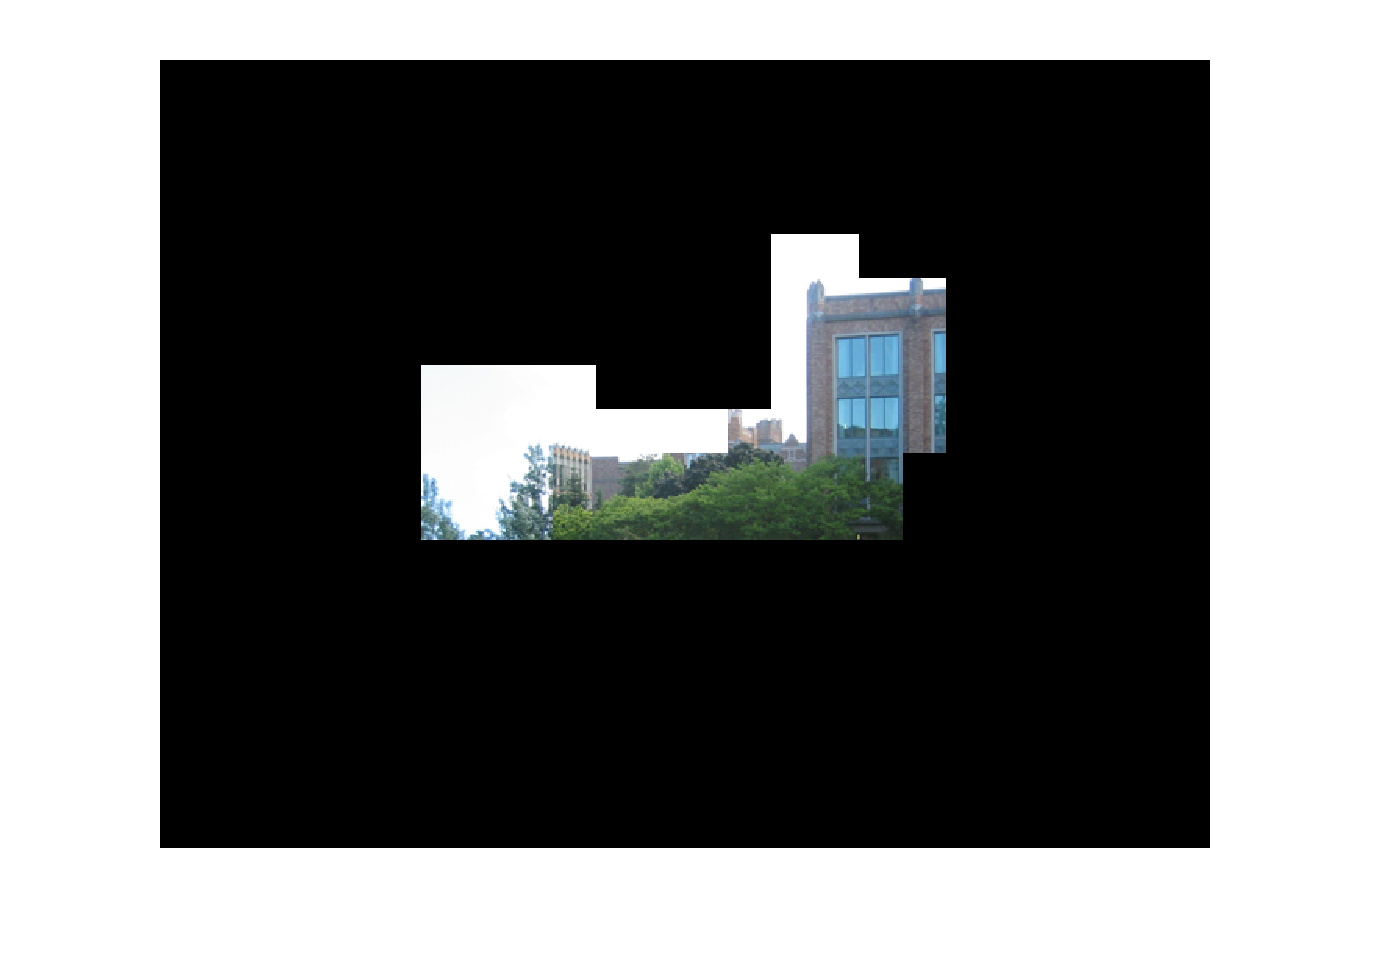
\includegraphics[height=0.25\textheight]{fig/algo_start.eps}
% \label{fig:placement1}}
% \hfil
%     \subfloat[The puzzle is constructed piece by piece.]{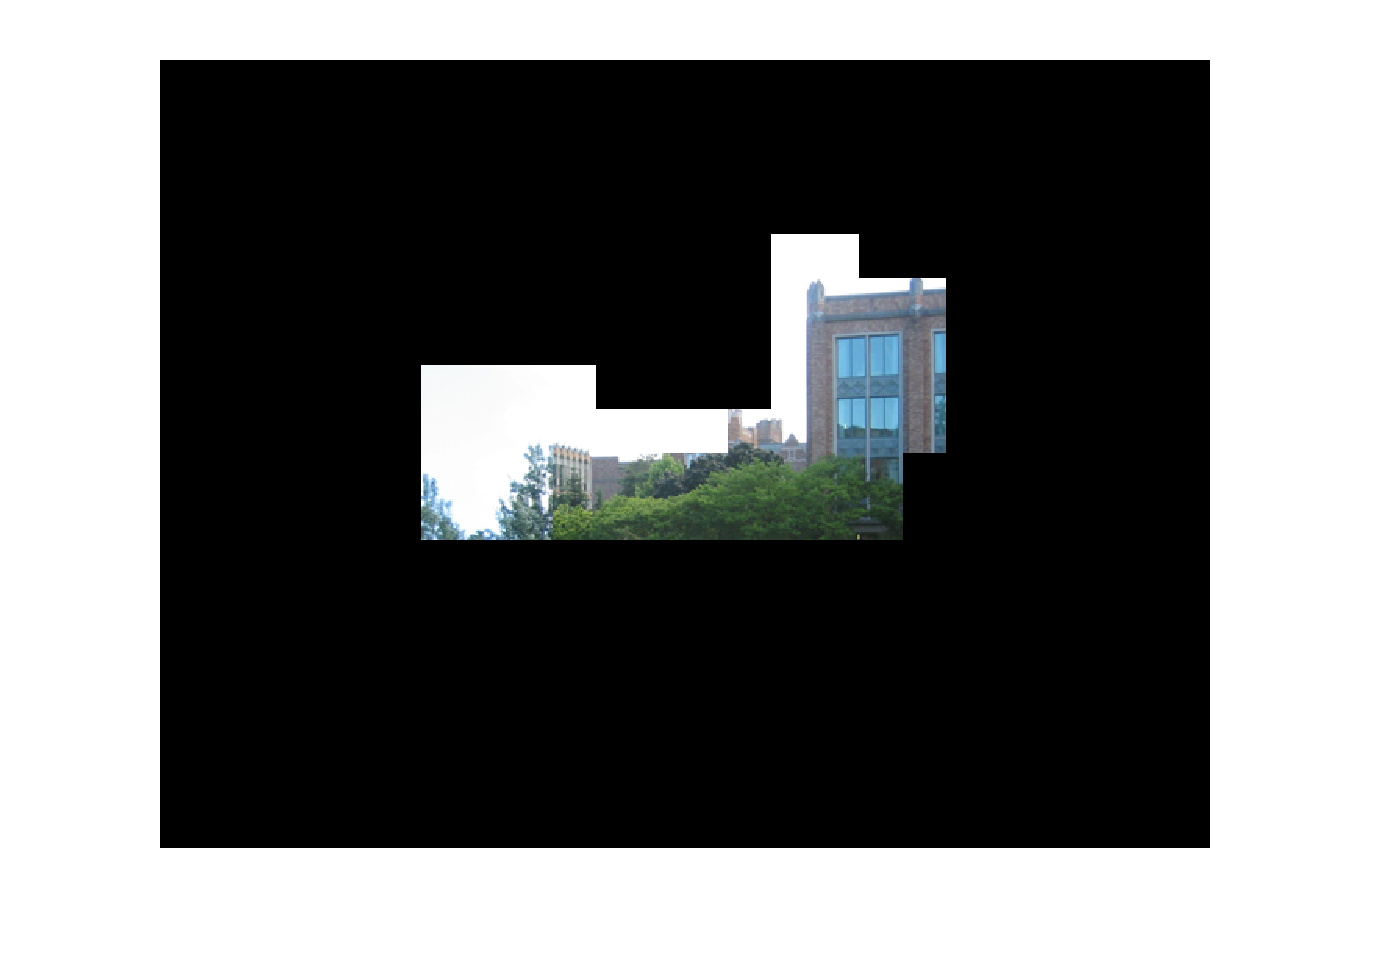
\includegraphics[height=0.25\textheight]{fig/algo_start.eps}
% \label{fig:placement1}}
% \hfil
%     \subfloat[The puzzle is constructed piece by piece.]{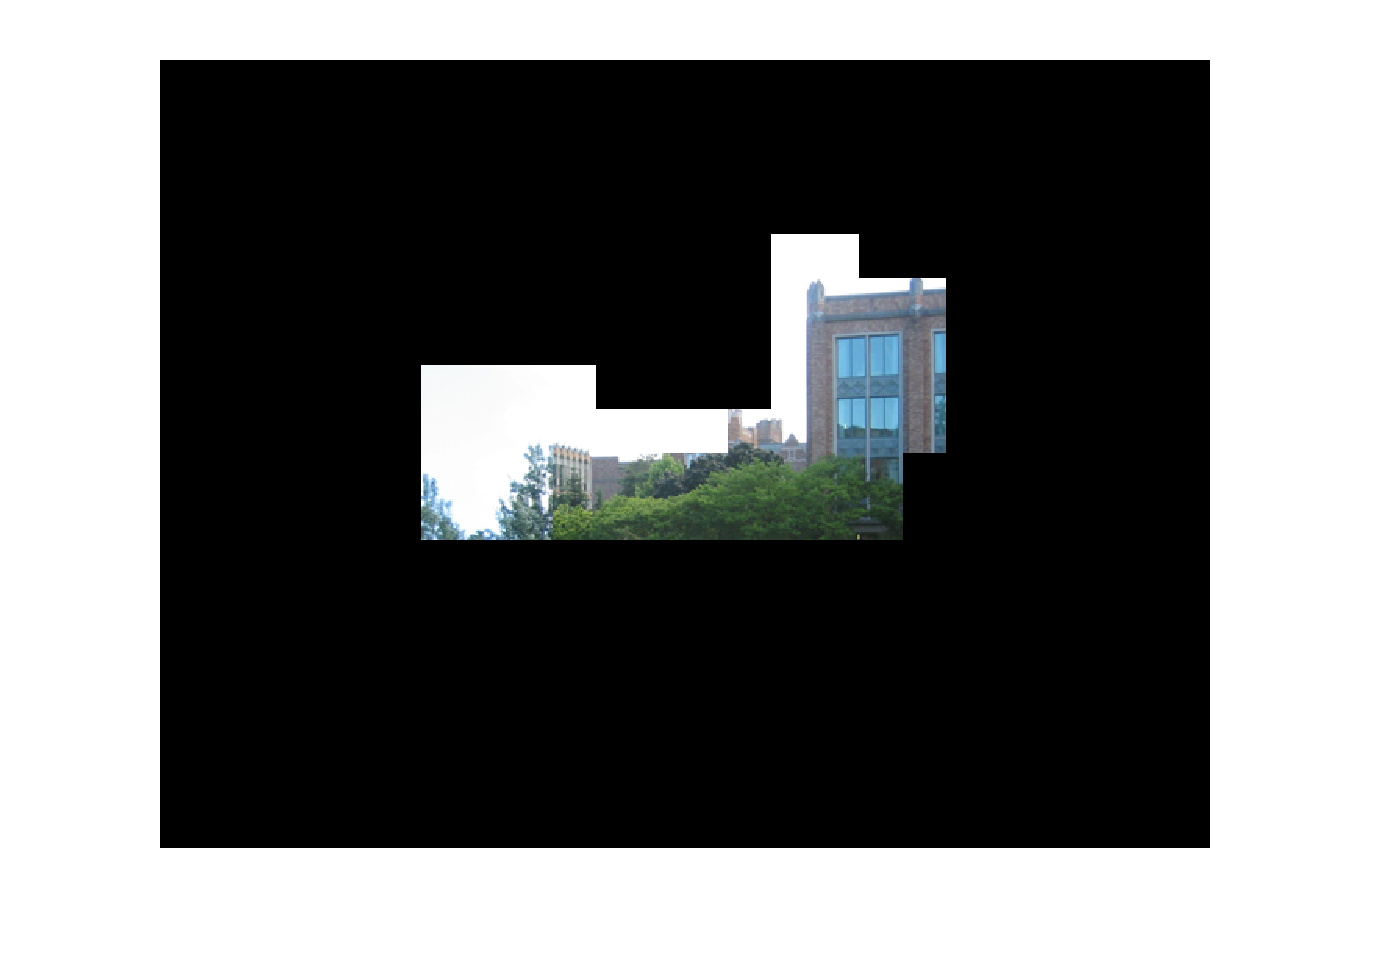
\includegraphics[height=0.25\textheight]{fig/algo_start.eps}
% \label{fig:placement1}}
% \hfil
%     \subfloat[The puzzle is constructed piece by piece.]{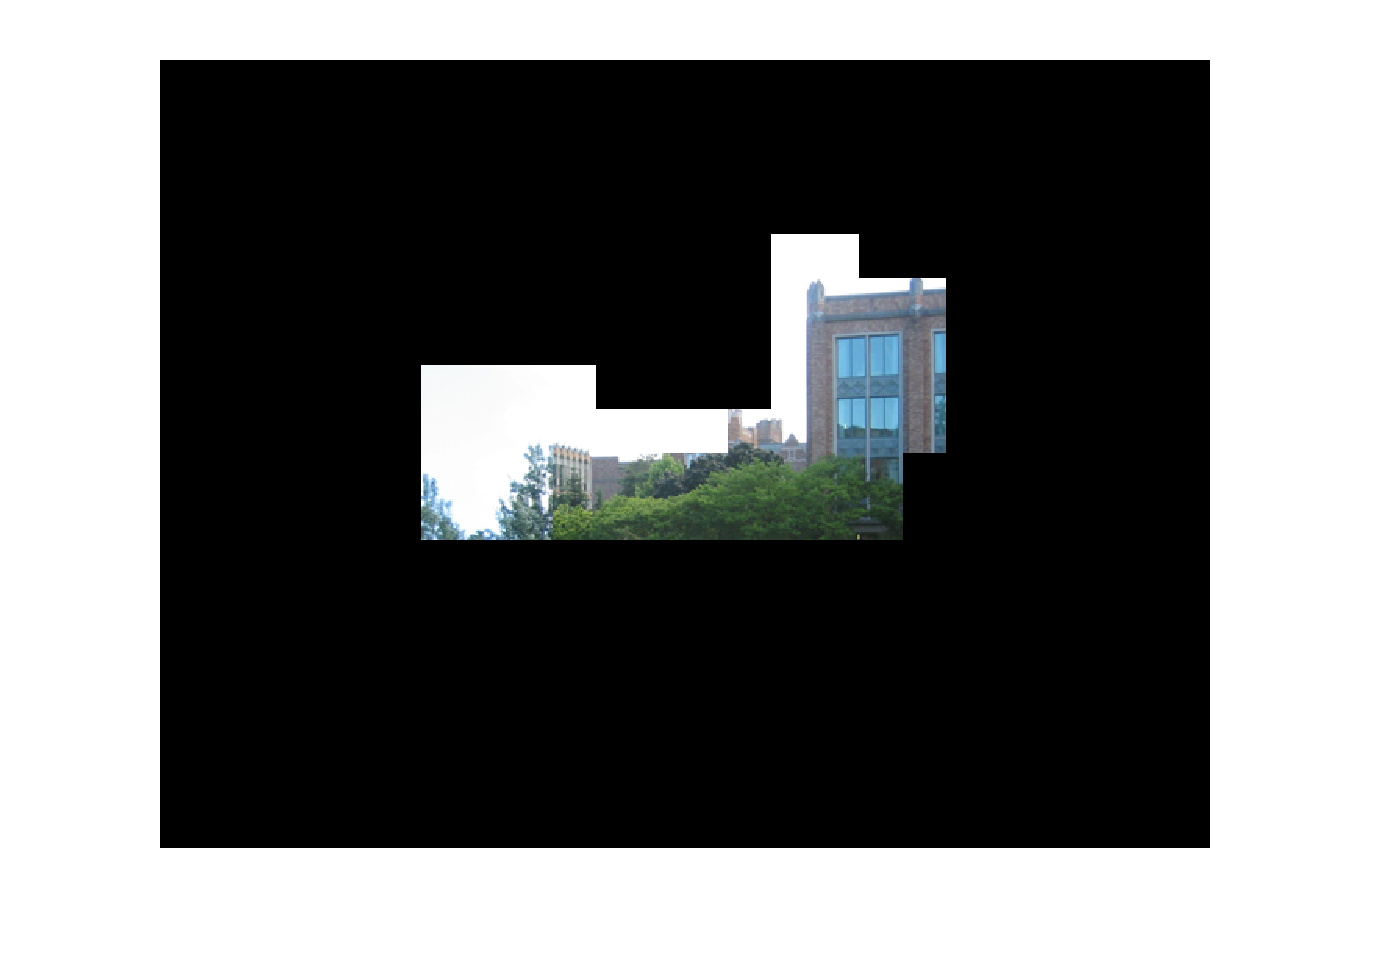
\includegraphics[height=0.25\textheight]{fig/algo_start.eps}
% \label{fig:placement1}}
% \hfil
    \begin{subfigure}{0.25\textheight}
        \centering
        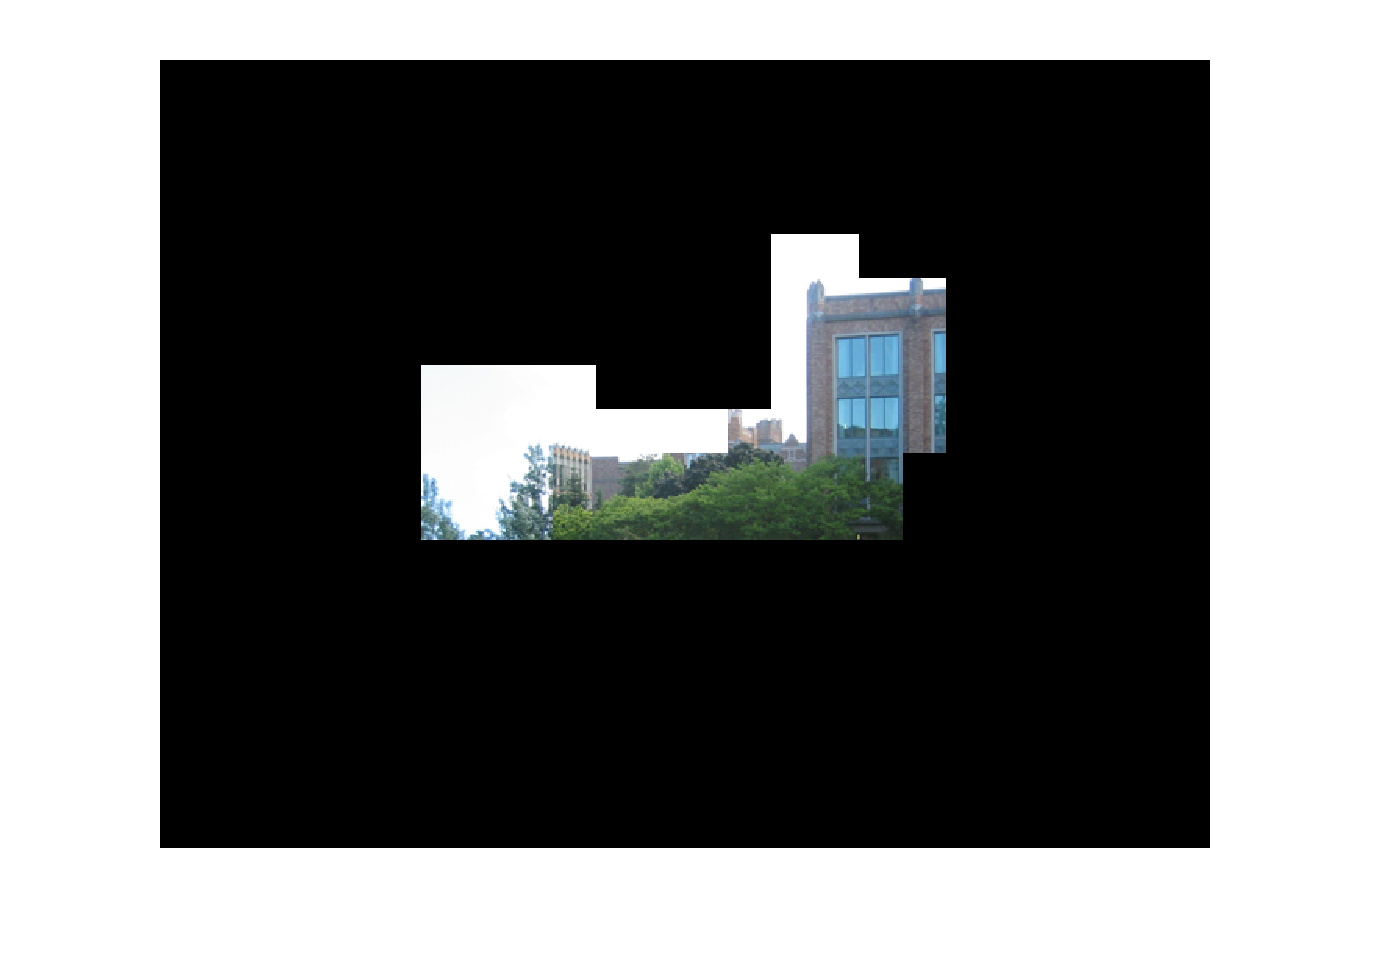
\includegraphics[width=\textwidth]{fig/algo_start.eps}
        \caption{The puzzle is constructed piece by piece.}    
        \label{fig:placement1}
    \end{subfigure}%
    
    \begin{subfigure}[b]{0.25\textheight}
        \centering
        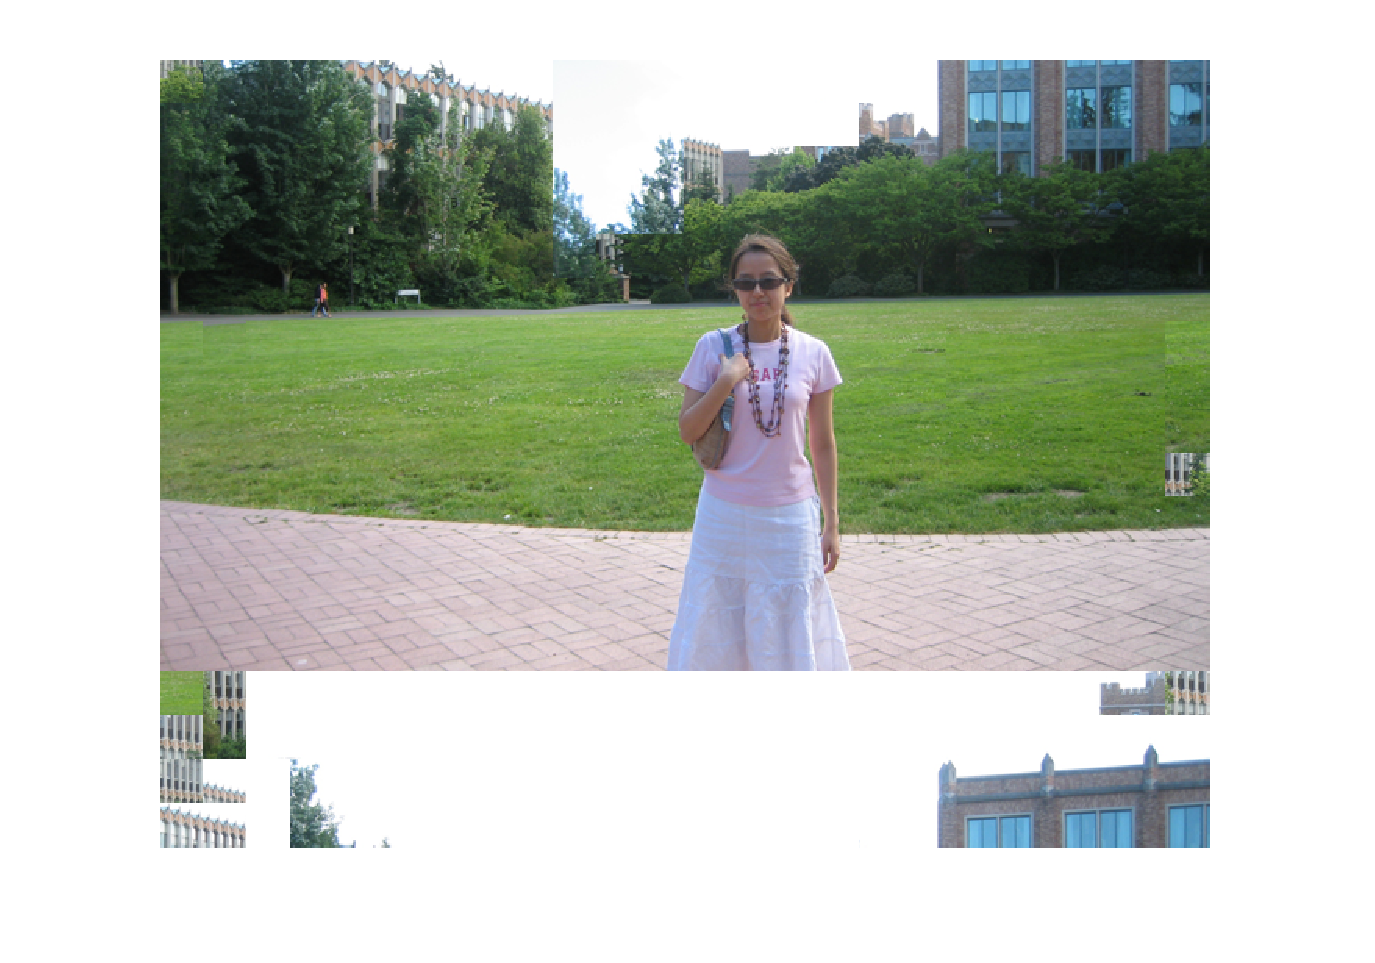
\includegraphics[width=\textwidth]{fig/algo_fin1.eps}
        \caption{At the end of the first placement phase, errors are present.}    
        \label{fig:placement2}
    \end{subfigure}%
    
    \begin{subfigure}[b]{0.25\textheight}
        \centering
        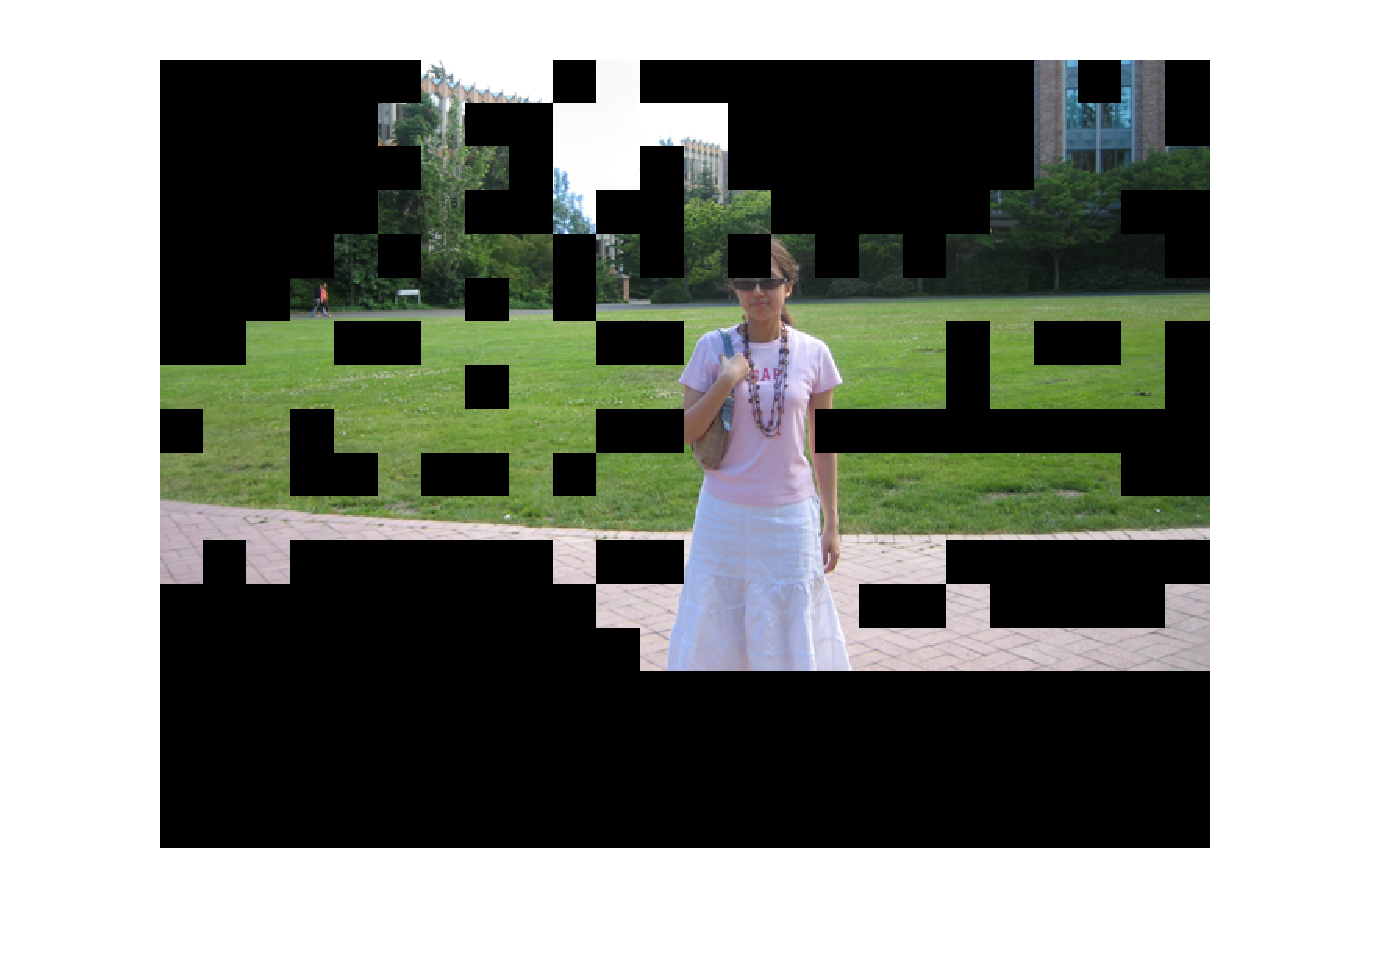
\includegraphics[width=\textwidth]{fig/algo_cut.eps}
        \caption{The biggest segment is extracted from the previous image and will serve as start for the next iteration.}    
        \label{fig:placement3}
    \end{subfigure}%
    
    \begin{subfigure}[b]{0.25\textheight}
        \centering
        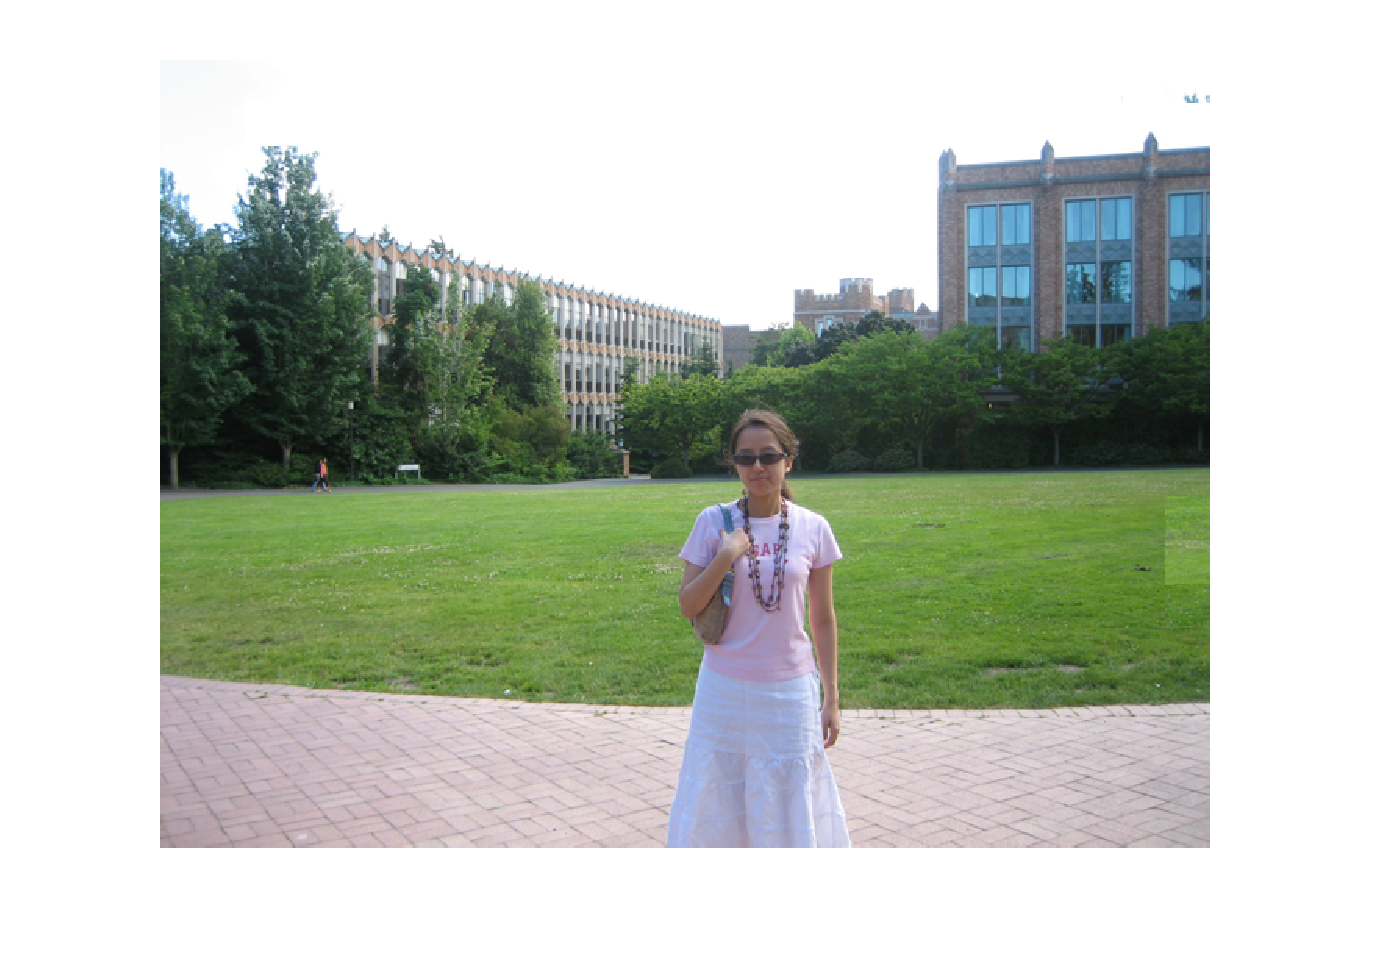
\includegraphics[width=\textwidth]{fig/algo_fin2.eps}
        \caption{The reconstruction is nearly perfect after two iterations.}    
        \label{fig:placement4}
    \end{subfigure}
    
    \caption{Illustration of the reconstruction algorithm}
    \label{fig:placement}
\end{figure}

The Matlab implementation of the algorithm was optimized using matrix computations, and the full solving of a 432 parts puzzle takes less than 10 seconds.

\section{Results}
\subsection{Metric parameters}

The parameters of the dissimilarity metrics are varied to determine which values give the best results. The methods were tested with different parameters on the set of images\footnote{available here: \url{http://people.csail.mit.edu/taegsang/Documents/jigsawCode.zip}} first used by Cho et al. \cite{cho} and then in \cite{robust} and \cite{greedy} for puzzle pieces of size 28 by 28 pixels. The number of pieces of the puzzle in then of 432. The error is expressed as the percentage of badly positioned pieces for all the 20 images of the set. 

\paragraph{M+S} \mbox{}

The parameter $r$ from \autoref{eq:ms} is varied from 1 to 20. The accuracy for each value is shown in \autoref{fig:ms}.

\begin{figure}[H]
\centering
% This file was created by matlab2tikz.
%
%The latest updates can be retrieved from
%  http://www.mathworks.com/matlabcentral/fileexchange/22022-matlab2tikz-matlab2tikz
%where you can also make suggestions and rate matlab2tikz.
%
\definecolor{mycolor1}{rgb}{0.00000,0.44700,0.74100}%
\definecolor{mycolor2}{rgb}{0.85000,0.32500,0.09800}%
\definecolor{mycolor3}{rgb}{0.92900,0.69400,0.12500}%
%
\begin{tikzpicture}

\begin{axis}[%
width=.8\linewidth,
height=.3\textheight,
at={(0.758in,0.481in)},
scale only axis,
xmin=0,
ylabel=Accuracy (\%),
xlabel= $r$ parameter,
axis background/.style={fill=white},
legend style={legend cell align=left, align=left, draw=white!15!black},
cycle list name=exotic
]

\addplot table [col sep=comma]{data/param_ms.csv};

\end{axis}
\end{tikzpicture}%
\caption{Performance of the M+S for various values of the $r$ parameter}
\label{fig:ms}
\end{figure}

The accuracy is maximum for $r=16$, hence this value will be retained for the final solver. This is also the value of $r$ that yielded the best results in \cite{robust}, which confirms this experimental result.

\paragraph{M+pq} \mbox{}

The parameter $r$ from \autoref{eq:mpq} is varied. The accuracy for each value is shown in \autoref{fig:param_pq}.


\begin{figure}[H]
\centering
% This file was created by matlab2tikz.
%
%The latest updates can be retrieved from
%  http://www.mathworks.com/matlabcentral/fileexchange/22022-matlab2tikz-matlab2tikz
%where you can also make suggestions and rate matlab2tikz.
%
\definecolor{mycolor1}{rgb}{0.00000,0.44700,0.74100}%
\definecolor{mycolor2}{rgb}{0.85000,0.32500,0.09800}%
\definecolor{mycolor3}{rgb}{0.92900,0.69400,0.12500}%
%
\begin{tikzpicture}

\begin{axis}[%
width=.8\linewidth,
height=.3\textheight,
at={(0.758in,0.481in)},
scale only axis,
xmin=0,
ylabel=Accuracy (\%),
xlabel= $r$ parameter,
axis background/.style={fill=white},
legend style={legend cell align=left, align=left, draw=white!15!black},
cycle list name=exotic
]

\addplot table [col sep=comma]{data/param_pq.csv};

\end{axis}
\end{tikzpicture}%
\caption{Performance of the M+pq for various values of the $r$ parameter}
\label{fig:param_pq}
\end{figure}

When the $(L_p)^q$ is combined with the MGC, the best results are obtained when $r=9$, which will be retained. This M+pq combination has not been used in the literature, so that this conclusion only relies on the present experiments.

For both the M+S and the M+pq, the performance appears to be better when the contribution from the MGC is more significant than the contribution of the methods based on the pixel intensities.

\subsection{Performance comparison}

The metrics with optimal parameters are then used again on the same set of images. Their performance is compared for piece sizes of 84 by 84 pixels, 56 by 56 pixels and 28 by 28 pixels.

\begin{figure}[H]
    \centering
    \begin{tikzpicture}

\begin{axis}[%
ybar,
ymin = 0,
ymax = 100,
width=.75\linewidth,
height=0.25\textheight,
xticklabels={SSD,Lpq,MGC,M+S,M+pq},
xtick=data,
ylabel=Accuracy (\%),
at={(1.733in,1.051in)},
scale only axis,
]
\addplot table [col sep=comma]{data/dat84.csv};
\end{axis}
\end{tikzpicture}%
%\end{document}
    \caption{Performance comparison for bloc sizes of 84 pixels. The MGC is outperforming all others with an accuracy of 93.2\%.}
    \label{fig:perf84}
\end{figure}

The results for pieces of 84 by 84 pixels are shown in \autoref{fig:perf84}. When the size of the piece has a relatively high value, the solver is very accurate. As expected, the $(L_p)^q$ metric is performing better than the SSD as it has a very similar working principle but penalizes less the natural steep edges at the boundaries of the pieces. Surprisingly, the MGC is outperforming the more advanced M+S and M+pq metrics. The additional information brought by the pixel intensities degrades the information brought by the color gradients.

\begin{figure}[H]
    \centering
    \begin{tikzpicture}

\begin{axis}[%
ybar,
ymin = 0,
ymax = 100,
width=.75\linewidth,
ylabel=Accuracy (\%),
height=0.25\textheight,
xticklabels={SSD,Lpq,MGC,M+S,M+pq},
xtick=data,
at={(1.733in,1.051in)},
scale only axis,
]
\addplot table [col sep=comma]{data/dat56.csv};
\end{axis}
\end{tikzpicture}%
%\end{document}
    \caption{Performance comparison for bloc sizes of 56 pixels. The M+S is outperforming all others with an accuracy of 87.2\%.}
    \label{fig:perf56}
\end{figure}


It is worth noting that a mean accuracy of 90\% does not indicate in this case that each puzzle is reconstructed with 10\% of errors. Actually, most images are reconstructed very well, but a few of them are not accurately at all, dropping the mean.

The tendencies observed above are not true anymore when the size of the puzzle pieces goes down. In \autoref{fig:perf56} are shown the results for 54 by 54 pixels pieces, where it appears that the M+S is the most accurate method. When the border is smaller, less information is available and the combination of the color and gradient information allows to get more accuracy. An unexpected observation is that even if the SSD alone is far from being as accurate as the $(L_p)^q$, the combination of the SSD and the MGC outperforms the combination of the $(L_p)^q$ and the MGC.

\begin{figure}[H]
    \centering
    \begin{tikzpicture}

\begin{axis}[%
ybar,
ymin = 0,
ymax = 100,
width=.75\linewidth,
height=0.25\textheight,
xticklabels={SSD,Lpq,MGC,M+S,M+pq,\cite{greedy},\cite{Gallagher},\cite{robust}},
ylabel=Accuracy (\%),
xtick={1,...,8},
at={(1.733in,1.051in)},
scale only axis,
]
\addplot table [col sep=comma]{data/dat28.csv};
%\addplot+[ybar] plot coordinates
	%{(6,94) (7,95.3) (8,95.6)};
\end{axis}
\end{tikzpicture}%
%\end{document}
    \caption{Performance comparison for bloc sizes of 28 pixels. The M+S is outperforming all others with an accuracy of 66.3\%.}
    \label{fig:perf28}
\end{figure}

Lastly, the solver was tested on small pieces of 28 by 28 pixels. The side of the pieces being very small, there is little information available and the accuracy drops to 66\%. Still, the M+S metric is the one outperforming the others, and the conclusions from the 56 by 56 case hold.


\section{Conclusion}
Based on the quite active research on the subject of automatic puzzle solving, several dissimilarity metrics have been introduced. The SSD and the $(L_p)^q$) are based on the color intensities at the boundaries of the pieces and the MGC is based on the gradient of these intensities. The two types of dissimilarity estimations can be combined into the M+S and the M+pq.

A placement algorithm has been developed, whose objective was to reconstruct the puzzle based on the dissimilarity between all the pieces of the puzzles in all the possible configurations. To lower the number of errors due to the placement, a segment of symmetric matches is extracted at the end of the placement and will serve as a start for the next iteration.

A set of images widely used in the literature has been used first to tune the parameters of the metrics, and next to quantify the performance of the puzzle solver. An accuracy of 93\% was reached on puzzles composed of pieces of 84 by 84 pixels using the MGC method. For lower sizes, the M+S method is the best one, and the accuracy to 87\% for 56 by 56 and to 66\% for 28 by 28.

The code is implemented in Matlab, and C/MEX functions are available to fasten the execution.

Performance could be improved at both phases of the reassembly. Firstly, the dissimilarity metrics could be improved to use more information than the content of the border only. Prediction-based or probabilistic metrics also exist. Secondly, the placement algorithms used in the literature are a bit more involved.

The jigsaw puzzle problem stays an open problem as no one has yet came up with a solver able to reconstruct any puzzle with 100\% accuracy.


\appendix

The work separation was done as follows: \begin{itemize}
    \item Mathieu Petitjean did the research of the existing techniques for computing the dissimilarity between pieces and implemented them in Matlab.
    
    \item Cédric Hannotier implemented the iterative placement algorithm on the basis of theses dissimilarity measures. He also optimized the Matlab code to reach fast execution time.
    
    \item Victor Artois ran the expirements to determine the optimal values of the parameters and compared the performance of the prosposed metrics for various puzzle sizes.
\end{itemize}

\ifCLASSOPTIONcaptionsoff
  \newpage
\fi

\printbibliography

\end{document}


